\documentclass{report}
\usepackage{graphicx}
\usepackage{xepersian}
\usepackage{geometry}
\settextfont[Scale=1.2]{XB Zar}
\renewcommand{\baselinestretch}{1.8}


% absolute position title
\usepackage{textpos}

% section numbering
\renewcommand{\thesection}{\arabic{section}}
\renewcommand{\thesubsection}{\thesection.\arabic{subsection}}
\renewcommand{\thesubsubsection}{\thesection.\arabic{subsection}.\arabic{subsubsection}}

\title{
\begin{normalsize}
به نام خدا
\end{normalsize}
\\[2cm]
بررسی مقاله
\\[1cm]
واسنجی سریع دوربین برای تحلیل ویدئوهای ورزشی
}
\author{یاسر سوری
\\
\\ \small دانشگاه صنعتی شریف
\\ \small souri@ce.sharif.edu
}
\begin{document}
\maketitle
%\begin{textblock*}{15cm}(0cm,-8cm)\centering به نام خدا \end{textblock*}

\begin{abstract}
این مقاله\cite{new_paper} نسخه‌ی سریع‌تر مقاله‌ی قبلی\cite{old_paper} توسط همین نویسنده است. در این مقاله سعی شده است که سرعت واسنجی تا حد بلادرنگ افزایش یابد. کلیت الگوریتم نسبت به نسخه‌ی قبلی حفظ شده است، ولی اجزای مختلف با اجزایی با کارایی بهتر جایگزین شده است. فرضیات این مقاله مثل فرضیات مقاله‌ی قبلی است و از این نظر با هم تفاوتی ندارند.

\end{abstract}

\section{فرض‌های مسئله}
در این بخش بعضی از فرضیات مسئله‌ای که قرار است در این مقاله حل شود مورد بررسی قرار می‌گیرد.
\begin{itemize}
\item
فرض شده است که، پارامتر‌های هشتگانه ماتریس هوموگرافی بین زمین و تصویر دوربین را بدست می‌آوریم، و پارامترهای \lr{pan}، \lr{tilt} و \lr{zoom} به صورت مجزا محاسبه نمی‌شوند.
\item
همچنین، پارامترهای مکان دوربین، \lr{roll} و \lr{lens distortion} در طول زمان تغییر نمی‌کنند.
\item
مدل زمین ورزشی (شامل خط‌های زمین، طول و فاصله‌ی آن‌ها از هم) را می‌دانیم.
\end{itemize}
\section{کلیت روش}
\begin{enumerate}
\item \textbf{تشخیص نقاط روی خطوط مدل زمین}

فرض می‌کینم که رنگ نقاط روی خطوط مدل زمین در واقع سفید است. همچنین باید دقت شود که دیگر نقاط سفید، برای مثال لباس بازیکنان و یا قسمت‌هایی از ورزشگاه به عنوان نقاط سفید روی خط تشخیص داده نشود.
\item \textbf{حدس پارامترهای خط}

با استفاده از خروجی تشخیص دهنده‌ی نقاط سفید رو خطوط، در این مرحله باید پارامترهای خطوط را حدس بزنیم. برا یان کار از یک حدس‌زننده خط بر اساس \lr{RANSAC} استفاده می‌شود. همچنین در این مرحله به جای خطوط نامتناهی، پاره خط‌ها تشخیص داده می‌شوند. دانستن نقاط دو سر پاره خط، سرعت مرحله‌ی برازش مدل را افزایش می‌دهد.
\item \textbf{برازش مدل}

خروجی مرحله‌ی قبل تعدادی خط است که از تصویر دوربین استخراج شده است. حال می‌خواهیم تشخیص دهیم که هر کدام از این خطوط مربوط به کدام خط از مدل زمین ورزشی است. این قسمت توسط یک بهینه‌سازی ترکیبی انجام می‌شود، که در حالت‌های مختلف انطباق بین خطوط مدل و تصویر، امتحان و ارزیابی می‌شود. 

دو روش جستجو در این قسمت تعبیه شده است: ابتدا جستجو توسط دو پاره خط. این روش سریع است،‌ولی در همه‌ی حالت‌ها پاسخ ندارد و اگر این جستجو پاسخی نداشته باشد از روش بعدی استفاده می‌شود. جستجوی دوم با استفاده از دو جفت خط (نامتناهی) است، که نسبت به روش اول مقاوم‌تر است ولی کند است و تنها در حالتی که روش اول پاسخ ندهد از این روش استفاده می‌کنیم.
\item \textbf{دنبال کردن}

در این مقاله این بخش مطرح نشده است. به عبارت دیگر این قسمت دقیقا مانند مقاله‌ی قبلی\cite{old_paper} است.
\end{enumerate}

در آغاز گام‌های ۱ تا ۳ انجام می‌شوند، تا مکان اولیه‌ی مدل زمین در تصویر بدست آید. پس از آن برای تصاویر بعدی، فقط گام‌های ۱ و ۴ انجام می‌شود.

\section{جزئیات الگوریتم}
\subsection{تشخیص نقاط سفید روی خطوط مدل زمین}
تشخیص نقاط سفید روی خطوط مدل زمین دو گام دارد:
\begin{itemize}
\item \textbf{گام اول}: 
این گام ساده و سریع است و عبارت است از یک حد آستانه برای درخشندگی و یک شرط حد آستانه دیگر برای حذف قسمت‌های بزرگ و سفید (مثل لباس بازیکنان). برای جزئیات این بخش به مقاله‌ی قبل مراجعه\cite{old_paper} شود.
\item \textbf{گام دوم}: 
این گام از نقاط سفیدی که در قسمت‌های دارای بافت هستند صرف نظر می‌کند. این قسمت کند است ولی حاصل را دقیق‌تر می‌کند. برای جزئیات این بخش به مقاله‌ی قبل مراجعه\cite{old_paper} شود.
\end{itemize}
می‌دانیم که از بخش تشخیص‌دهنده‌ی نقاط سفید هم در مقداردهی اولیه و هم در دنبال کردن استفاده می‌شود. در مقداردهی اولیه زمان برای ما اهمیت ندارد بلکه دقت مهم است و در دنبال کردن زمان برای ما اهمیت دارد. به همین خاطر در مقدار دهی اولیه از هر دو گام و در دنبال کردن فقط از گام اول استفاده می‌کنیم.
\subsection{حدس پارامترهای خط}
حال که نقاط روی خطوط مدل را استخراج کردیم، لازم است که معادله‌ی پارامتری خطوط را استخراج کنیم. ابتدا از یک الگوریتم مثل \lr{RANSAC} استفاده می‌کنیم تا خط غالب را از بین مجموعه نقاط استخراج کنیم. سپس نقاط دو سر پاره خط تشخیص داده می‌شوند و پس از آن پارامترهای خط باز مجددا توسط یک تقریب‌زن \lr{least-squares} بهبود می‌یابد.

سپس نقاط سفیدی را که در راستای پاره خط و خارج از دو سر آن هستند حذف می‌شنوند. این کار را آن‌قدر ادامه می‌دهیم تا دیگر خطی را نتوان پیدا کرد.

\sebsection{برازش مدل}
در این مرحله دو الگوریتم معرفی شده است: برازش سریع (که جدید است) و برازش مقاوم (از مقاله فبلی).
\begin{figure}
\centering
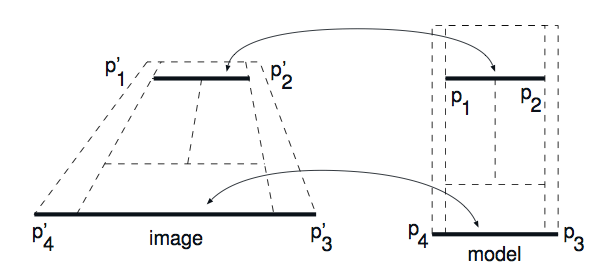
\includegraphics[scale=0.5]{fast_fitting.png}
\caption{برازش سریع}
\label{fast_fitting}
\end{figure}
در برازش سریع از دو پاره خط کخ در تصویر تشخیص داده شده است استفاده می‌شود و پاره‌خط‌های  نظیر آن دو در مدل تشخیص داده می‌شوند. (به شکل \ref{fast_fitting} توجه شود)

\begin{latin}
\bibliography{court_model_bib}{}
\bibliographystyle{plain}
\end{latin}

\end{document}